\documentclass{ieeeaccess}
\usepackage{cite}
\usepackage{amsmath,amssymb,amsfonts}
\usepackage{algorithmic}
\usepackage{graphicx}
\usepackage{textcomp}

\usepackage{bm}
\makeatletter
\AtBeginDocument{\DeclareMathVersion{bold}
\SetSymbolFont{operators}{bold}{T1}{times}{b}{n}
\SetSymbolFont{NewLetters}{bold}{T1}{times}{b}{it}
\SetMathAlphabet{\mathrm}{bold}{T1}{times}{b}{n}
\SetMathAlphabet{\mathit}{bold}{T1}{times}{b}{it}
\SetMathAlphabet{\mathbf}{bold}{T1}{times}{b}{n}
\SetMathAlphabet{\mathtt}{bold}{T1}{pcr}{m}{n}
\SetSymbolFont{symbols}{bold}{OMS}{cmsy}{b}{n}
\renewcommand\boldmath{\@nomath\boldmath\mathversion{bold}}}
\makeatother

\def\BibTeX{{\rm B\kern-.05em{\sc i\kern-.025em b}\kern-.08em
    T\kern-.1667em\lower.7ex\hbox{E}\kern-.125emX}}

%Your document starts from here ___________________________________________________
\begin{document}
\history{Date of publication xxxx 00, 0000, date of current version xxxx 00, 0000.}
\doi{10.1109/ACCESS.2024.0429000}

\title{Preparation of Papers for IEEE ACCESS}
\author{\uppercase{First A. Author}\authorrefmark{1}, \IEEEmembership{Fellow, IEEE},
\uppercase{Second B. Author}\authorrefmark{2}, and Third C. Author,
Jr.\authorrefmark{3},
\IEEEmembership{Member, IEEE}}

\address[1]{National Institute of Standards and
Technology, Boulder, CO 80305 USA (e-mail: author@boulder.nist.gov)}
\address[2]{Department of Physics, Colorado State University, Fort Collins,
CO 80523 USA (e-mail: author@lamar.colostate.edu)}
\address[3]{Electrical Engineering Department, University of Colorado, Boulder, CO
80309 USA}
\tfootnote{This paragraph of the first footnote will contain support
information, including sponsor and financial support acknowledgment. For
example, ``This work was supported in part by the U.S. Department of
Commerce under Grant BS123456.''}

\markboth
{Author \headeretal: Preparation of Papers for IEEE TRANSACTIONS and JOURNALS}
{Author \headeretal: Preparation of Papers for IEEE TRANSACTIONS and JOURNALS}

\corresp{Corresponding author: First A. Author (e-mail: author@ boulder.nist.gov).}


\begin{abstract}
These instructions give you guidelines for preparing papers for
IEEE Access. Use this document as a template if you are
using \LaTeX. Otherwise, use this document as an
instruction set. The electronic file of your paper will be formatted further
at IEEE. Paper titles should be written in uppercase and lowercase letters,
not all uppercase. Avoid writing long formulas with subscripts in the title;
short formulas that identify the elements are fine (e.g., "Nd--Fe--B"). Do
not write ``(Invited)'' in the title. Full names of authors are preferred in
the author field, but are not required. Put a space between authors'
initials. The abstract must be a concise yet comprehensive reflection of
what is in your article. In particular, the abstract must be self-contained,
without abbreviations, footnotes, or references. It should be a microcosm of
the full article. The abstract must be between 150--250 words. Be sure that
you adhere to these limits; otherwise, you will need to edit your abstract
accordingly. The abstract must be written as one paragraph, and should not
contain displayed mathematical equations or tabular material. The abstract
should include three or four different keywords or phrases, as this will
help readers to find it. It is important to avoid over-repetition of such
phrases as this can result in a page being rejected by search engines.
Ensure that your abstract reads well and is grammatically correct.
\end{abstract}

\begin{keywords}
Enter key words or phrases in alphabetical
order, separated by commas. Autocorrelation, beamforming, communications technology, dictionary learning, feedback, fMRI, mmWave, multipath, system design, multipath, slight fault, underlubrication fault.
\end{keywords}

\titlepgskip=-21pt

\maketitle

% Contribuições: A ideia principal deste trabalho é evaluar diversos algoritmos disponíveis na literatura recente em um problema unificado de Séries Temporais.
% Por quê? (Contextualização) Fisgar o leitor com informações de senso comum que o levem a entender o contexto geral em que o trabalho se aplica. Urban Computing - Social Computing - Urban Data Science - Urban Data Mining - Urban Data Analysis - Urban Data Analytics - Urban Data Engineering - Urban Data Classification - Urban Data Clustering
% Trabalhos anteriores: o que foi inspiração para este trabalho? (Revisão da Literatura) - Bake off redux: a review and experimental evaluation of recent time series classification algorithms e Trabalho do Leonardo (Extraction and Exploration of Business Categories Signatures)

% Começar com frase que qualquer um da área consegue entender. Não focar direto no que o trabalho é, mas sim dar um contexto.
% Frases genéricas para a pessoa entender o tema, importãncia, motivação, etc.
% Apontar o problema.
% Por que não está solucionado?
% Explicar o que foi feito para solucionar o problema.
% Apresenta a estrutura geral do artigo.
% Problema em dataset do mundo real e entender como a regionalidade influencia no comportamento dos time series e na performance de classificadores.
\section{Introduction}
\label{sec:introduction}
\PARstart{}{} Urban environments have their own dynamics, comprised of a complex network of interactions between people, establishments, and infrastructure. Also, with the growth of technologies such as smartphone devices and Internet access, the amount of data generated in urban areas has increased significantly, providing valuable insights into the behavior of people in these environments. This data can be used to optimize urban services, improve resource management, and enhance the quality of life for residents.

Cities are systems that are constantly changing and evolving. One of the mais characteristics of an urban city is the diversity of establishments and services available to residents and visitors. These establishments, such as restaurants, cafes, and shops, attract people at different times of the day, creating patterns of occupancy that can be observed and analyzed.

Therefore, each city has its own characteristics and behaviors that can be observed along the time, which can be influenced by factors such as culture, climate, and local events. Different cities may have different patterns of occupancy for the same type of establishment, while different establishments may have similar patterns across different cities. These are some examples of how regional characteristics can influence the behavior of time series data and how challenging it can be to model and classify these patterns.

In Computer Science, the study of urban environments is known as Urban Computing. It involves collecting, combining, and analyzing vast and diverse datasets produced by various sources within city environments \cite{zheng2014urban}.
One of the main sources of data in urban environments is the Popular Times dataset from Google, which provides information about the popularity of establishments at different times of the day. This dataset is generated from aggregated and anonymized data from users who have opted to share their location history with Google. The dataset contains information about the popularity of establishments such as restaurants, cafes, and shops, based on the number of visitors at different times of the day.

%\textbf{TODO: incluir contribuições do trabalho}

Time Series Classification (TSC) is a subfield of time series analysis that focuses on the classification of time series data. The goal of TSC is to develop algorithms that can accurately classify time series data into different categories based on their temporal patterns. TSC has applications in a wide range of domains, including finance, healthcare, and environmental monitoring.

To address the challenges of TSC, several algorithms have been proposed in the literature. These algorithms vary in terms of their complexity, performance, and suitability for different types of time series data. Some of the most commonly used algorithms for TSC include Dynamic Time Warping (DTW), Long Short-Term Memory (LSTM) networks, and Convolutional Neural Networks (CNNs).

The performance of these algorithms can vary depending on the characteristics of the time series data and the specific problem being addressed. Therefore, it is important to evaluate the performance of different algorithms on a diverse set of time series datasets to identify the most effective approaches for TSC.

This type of study was conducted by Middlehurst et al. \cite{middlehurst2024bakeoff}, who compared the performance of different TSC algorithms on a set of benchmark datasets. The paper evaluates 18 Time Series Classification (TSC) algorithms evaluating a broad range of modern TSC algorithms, including traditional distance-based methods, feature-based approaches, and state-of-the-art deep learning techniques. 

Based on the Popular Times dataset extracted and studied by Silva et al. \cite{silva2019signatures}, where he extracted the Popular Times data from Google Maps for a set of establishments in different cities and countries, this study aims to continue his contributions by evaluating the performance of different time series classification algorithms on this dataset.
% Explanation of his study
%In their study, the authors structured the time series clustering experiments into three distinct stages. The first stage involved clustering the time series data of businesses within the same category to analyze intra-category behaviors. The second stage focused on clustering the signatures of different categories to explore whether multiple categories exhibit similar behaviors, potentially represented by a single signature. The same criterion used for determining the number of clusters in the first stage was applied here.

%The final stage aimed to identify country-level category signatures by associating similar category behaviors across cities within a country. To ensure representativeness, a category's behavior was considered characteristic of a country only if it was observed in all sampled cities. To achieve this, the number of clusters for country-level category signatures was constrained by the number of clusters found in the city with the fewest clusters for that category. This approach ensured consistency across the sampled cities when identifying representative country-level behaviors.
The authors divided the time series clustering experiments into three stages. First, they clustered time series of businesses within the same category to analyze intra-category behaviors. Second, they clustered signatures of different categories to identify shared behaviors, using the same clustering criteria as the first stage. Finally, they identified country-level category signatures by associating similar behaviors across cities, ensuring a behavior was representative of the country only if observed in all sampled cities. The number of clusters for country signatures was based on the city with the fewest clusters for that category.
% How am I going to continue his contribution? I am going to use his dataset to evaluate the performance of different time series classification algorithms. Also, compare the results based on some metrics. Accuracy,F1-Score, Precision and Recall. Need to explain the metrics and why I choose these.

% Como é o desempenho da classificação do Leonardo em relação a outros classificadores de Time Series? Quais são os classificadores que eu vou utilizar? Por que eu escolhi esses classificadores? O que eu espero encontrar com esses classificadores? Quais são as métricas que eu vou utilizar para avaliar o desempenho dos classificadores? Por que eu escolhi essas métricas? O que eu espero encontrar com essas métricas?
Studies [2] and [3] provided a foundation for addressing several questions. 
% Como a separação dos dados por cidade afeta a precisão do classificador? O que acontece ao treinar o classificador sem a separação dos dados por cidade ou país? Como a adição das colunas de cidade e país impacta a performance do modelo?
%A troca de países para teste e treinamento afeta a performance do modelo?
%Como a inclusão de muitas informações extraídas pelo tsfel afeta o desempenho dos classificadores?
%Qual é a diferença de desempenho entre os diferentes classificadores utilizados?
%Qual cenário produziu o melhor equilíbrio entre F1-score, precisão e recall?
%Em quais cenários o modelo teve maior taxa de overfitting ou underfitting?
%Qual foi o impacto das features temporais adicionais na performance do classificador?
 %Existem padrões de desempenho distintos dependendo das cidades ou países analisados?

% reescrever o parágrafo seguinte:

From their study, it was possible to select the best algorithms to be appied into the problem of time series classification with a real world dataset, the Popular Times dataset from Google.

\cite{middlehurst2024bakeoff}

% Ainda estou escrevendo o corpo da introdução, mas quero fechar a Introdução com algo nesta linha.

%In this study, the analysis of the dataset focuses on examining how people visit and interact with these establishments over time. 
%By observing patterns of occupancy at different times and types of establishments, the aim is to understand the variations in consumer behavior and how these patterns can be useful in predicting movement in different types of establishments. 
%Time series analysis provides a more detailed and accurate view of collective behavior over time, which can be used to predict the occupancy conditions of a location at certain times, optimizing resource management and improving the experience for both customers and establishment owners.

% Based on the time series from the Popular Times dataset, several tests were performed with different classifiers, with the aim of evaluating the predictive capacity of the models and identifying which would be the most effective in capturing the temporal patterns of popularity of establishments. 
% The choice of classifiers was inspired by a recent "bake-off redux" study (Bake off redux: a review and experimental evaluation of recent time series classification algorithms) that compared the performance of different classification approaches on time series datasets.
% “Bake-Off” is a term used in technology to describe a process where multiple technologies or tools are tested against each other to determine the best one. It includes evaluation of various factors such as efficiency, accuracy, and ease of use. 
% These classifiers were tested using the K-fold cross-validation technique, a process in which the data is divided into K parts, and each is used as a test set while the other K-1 parts are used for training, ensuring a robust evaluation of the models.

% In addition, the data was separated by city and country to test how the performance of the models would vary depending on the granularity of the information. This test was important to understand how temporal characteristics can behave differently in a specific city or in a national context. In the tests, the city and country variables were omitted to verify the ability of the models to identify patterns without the influence of this information, which can be useful to assess the robustness of the classifiers in different contexts.

% From these analyses, the results obtained help to better understand how time series of popularity can be modeled and used to generate useful predictions in contexts such as retail and establishment management. The study offers a significant contribution by applying time series models in the area of location and occupancy data analysis, and by exploring the applicability of the classifiers in real time data, such as that provided by Google.

%\textbf{TODO: incluir organização do trabalho}

%\subsection{Equations}
% Number equations consecutively with equation numbers in parentheses flush
% with the right margin, as in \eqref{eq}. To make your equations more
% compact, you may use the solidus (~/~), the exp function, or appropriate
% exponents. Use parentheses to avoid ambiguities in denominators. Punctuate
% equations when they are part of a sentence, as in
% \begin{equation}E=mc^2.\label{eq}\end{equation}

% The following 2 equations are used to test 
% your LaTeX compiler's math output. Equation (2) is your LaTeX compiler' output. Equation (3) is an image of what (2) should look like.
% Please make sure that your equation (2) matches (3) in terms of symbols and characters' font style (Ex: italic/roman).

% \begin{align*} \frac{47i+89jk\times 10rym \pm 2npz }{(6XYZ\pi Ku) Aoq \sum _{i=1}^{r} Q(t)} {\int\limits_0^\infty \! f(g)\mathrm{d}x}  \sqrt[3]{\frac{abcdelqh^2}{ (svw) \cos^3\theta }} . \tag{2}\end{align*}

% $\hskip-7pt$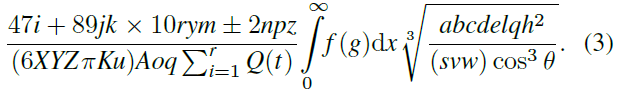
\includegraphics[scale=0.52]{equation3.png}

% Be sure that the symbols in your equation have been defined before the
% equation appears or immediately following. Italicize symbols ($T$ might refer
% to temperature, but T is the unit tesla). Refer to ``\eqref{eq},'' not ``Eq. \eqref{eq}''
% or ``equation \eqref{eq},'' except at the beginning of a sentence: ``Equation \eqref{eq}
% is $\ldots$ .''

% \subsection{LaTeX-Specific Advice}

% Please use ``soft'' (e.g., \verb|\eqref{Eq}|) cross references instead
% of ``hard'' references (e.g., \verb|(1)|). That will make it possible
% to combine sections, add equations, or change the order of figures or
% citations without having to go through the file line by line.

% Please don't use the \verb|{eqnarray}| equation environment. Use
% \verb|{align}| or \verb|{IEEEeqnarray}| instead. The \verb|{eqnarray}|
% environment leaves unsightly spaces around relation symbols.

% Please note that the \verb|{subequations}| environment in {\LaTeX}
% will increment the main equation counter even when there are no
% equation numbers displayed. If you forget that, you might write an
% article in which the equation numbers skip from (17) to (20), causing
% the copy editors to wonder if you've discovered a new method of
% counting.

% {\BibTeX} does not work by magic. It doesn't get the bibliographic
% data from thin air but from .bib files. If you use {\BibTeX} to produce a
% bibliography you must send the .bib files.

% {\LaTeX} can't read your mind. If you assign the same label to a
% subsubsection and a table, you might find that Table I has been cross
% referenced as Table IV-B3.

% {\LaTeX} does not have precognitive abilities. If you put a
% \verb|\label| command before the command that updates the counter it's
% supposed to be using, the label will pick up the last counter to be
% cross referenced instead. In particular, a \verb|\label| command
% should not go before the caption of a figure or a table.

% Do not use \verb|\nonumber| inside the \verb|{array}| environment. It
% will not stop equation numbers inside \verb|{array}| (there won't be
% any anyway) and it might stop a wanted equation number in the
% surrounding equation.

\section{The dataset} % TODO
% Nesta seção é importante descrever o dataset utilizado, como ele foi coletado, quais são as variáveis presentes, e como ele foi tratado para ser utilizado nos experimentos. Basicamente o meu dataset é o Popular Times do Google oriundo do trabalho de Silva et al.
Deepening into the dataset used in this work, the Popular Times dataset from Google was used. This dataset was collected by Silva et al. \cite{silva2019signatures}, and it contains information about the popularity of establishments at different times of the day. The popularity of the establishments in Google is also known as Popular Times.
The data was collected from a web crawler and processed with business names, categories, cities and coutries. Since their goal was to identify patterns of the Popular Times data of businesses related to food and drink consumption, they filtered the data to include only businesses in the categories of restaurants, bars, coffee shops, dance clubs (nightclubs) and bakeries. 
This specification was made to ensure that the data would be consistent and relevant to the study.
Within the data extraction, they used the HTML information to gather the Popular Times data in a hourly basis extracting the popularity values for each day of the day. The data was normalized to a scale of 0 to 1, where 0 represents the lowest popularity and 1 the highest popularity. 
The popularity values were modeled as a discrete sequence $v_k$, normalized between 0 and 1, where $k$ represents each hour of the day. This allowed the definition of a time series of popularity $S$ as:

\[
S = \{ v_k \mid \forall k \in [0, 23], \ 0 \leq v_k \leq 1 \},
\]

where $v_k$ denotes the normalized popularity at hour $k$. For each establishment, two distinct time series were generated using the Dynamic Time Warping Barycenter Averaging (DBA) technique: one representing the typical pattern on weekdays and the other representing the pattern on weekends.

Within this study, the dataset specialization was focused on weekdays only. This was done to ensure that the data would be consistent and relevant to the study since the behavior of establishments on weekdays can differ from weekends. 

\section{Methodology}
\label{sec:methodology}

The methodology of this research is designed to address the study of time series classification algorithms on the Popular Times dataset. 
The workflow consists of several steps, including algorithm selection, evaluation metrics, and experimental setup.
This section describes the dataset, preprocessing steps, classification algorithms, evaluation metrics, and experimental setup.

\subsection{Dataset Description}

The dataset used in this study consists of 12,704 rows and 28 columns, with each row representing an observation and each column providing a specific feature. 
The dataset includes time series data spanning 24 hours of the day, recorded at hourly intervals, along with contextual metadata, such as geographical and categorical information.

The features are structured as follows:
\begin{itemize}
    \item \textbf{Hourly Metrics:} Columns \texttt{h00} through \texttt{h23} represent normalized values corresponding to various metrics captured for each hour of the day. These hourly features reflect the dynamic behavior of specific entities over a full daily cycle.
    \item \textbf{Country and City Identifiers:} Two columns, \texttt{country} and \texttt{city}, provide geographical context for each observation, enabling analysis at different spatial scales.
    \item \textbf{Category Information:} The \texttt{category} column classifies the data into distinct groups based on the nature of the observed entities, facilitating category-specific analyses. It includes the categories of establishments such as restaurants, cafes, and bakeries.
\end{itemize}

%The dataset captures diverse patterns across various entities, with temporal dynamics reflected in the hourly metrics. 
%The normalized values for each hour are bounded between 0 and 1, ensuring uniform scaling and comparability across observations.

% Optional
\begin{table}[!h]
\caption{Sample Structure of the Dataset.}
\centering
\begin{tabular}{|c|c|c|c|}
\hline
\textbf{Column Name} & \textbf{Description} & \textbf{Type} & \textbf{Range/Values} \\ \hline
\texttt{h00--h23} & Hourly metrics (normalized) & Continuous & [0, 1] \\ \hline
\texttt{country} & Country identifier & Categorical & \textit{(e.g., 0, 1)} \\ \hline
\texttt{city} & City identifier & Categorical & \textit{(e.g., 0, 1, 2)} \\ \hline
\texttt{category} & Entity category & Categorical & \textit{(e.g., 0, 1, 2)} \\ \hline
\end{tabular}
\label{table:dataset_structure}
\end{table}

\section{Dataset Statistics}

This section provides a detailed breakdown of the dataset used in the study, covering counts by country, city, and categories, as well as distributions within each city and country.

\begin{table}[h!]
\centering
\caption{Count by Country}
\label{tab:count_by_country}
\begin{tabular}{|l|r|}
\hline
\textbf{Country} & \textbf{Count} \\
\hline
United States & 8218 \\
Brazil        & 4486 \\
\hline
\end{tabular}
\end{table}

\begin{table}[h!]
\centering
\caption{Count by City}
\label{tab:count_by_city}
\begin{tabular}{|l|r|}
\hline
\textbf{City}      & \textbf{Count} \\
\hline
New York & 3226 \\
Chicago & 2672 \\
San Francisco & 2320 \\
São Paulo & 2073 \\
Rio de Janeiro & 1324 \\
Curitiba & 1089 \\
\hline
\end{tabular}
\end{table}

\begin{table}[h!]
\centering
\caption{Count by Categories (Total)}
\label{tab:count_by_categories_total}
\begin{tabular}{|l|r|}
\hline
\textbf{Category}  & \textbf{Count} \\
\hline
Restaurants & 4837 \\
Bars        & 3752 \\
Coffee      & 1979 \\
Bakeries    & 1843 \\
Dance Clubs &  293 \\
\hline
\end{tabular}
\end{table}

\begin{table*}[h!]
\centering
\caption{Count by Categories in Each City}
\label{tab:count_by_categories_city}
\begin{tabular}{|l|r|r|r|r|r|r|}
\hline
\textbf{Category} & \textbf{Chicago} & \textbf{Curitiba} & \textbf{New York} & \textbf{Rio de Janeiro} & \textbf{San Francisco} & \textbf{São Paulo} \\
\hline
Bakeries    &  315 &  198 &  590 &  133 &  186 &  421 \\
Bars        &  827 &  212 &  877 &  398 &  758 &  680 \\
Coffee      &  595 &   16 &  770 &   46 &  447 &  105 \\
Dance Clubs &   54 &   14 &   89 &   20 &   57 &   59 \\
Restaurants &  881 &  649 &  900 &  727 &  872 &  808 \\
\hline
\end{tabular}
\end{table*}

\begin{table*}[h!]
\centering
\caption{Count by Categories in Each Country}
\label{tab:count_by_categories_country}
\begin{tabular}{|l|r|r|}
\hline
\textbf{Category} & \textbf{Brazil} & \textbf{United States} \\
\hline
Bakeries    &  752 & 1091 \\
Bars        & 1290 & 2462 \\
Coffee      &  167 & 1812 \\
Dance Clubs &   93 &  200 \\
Restaurants & 2184 & 2653 \\
\hline
\end{tabular}
\end{table*}
    

\begin{table}[h!]
\centering
\caption{Total Rows in Dataset}
\label{tab:total_rows}
\begin{tabular}{|l|r|}
\hline
\textbf{Metric} & \textbf{Count} \\
\hline
Total Rows  & 12704 \\
\hline
\end{tabular}
\end{table}

The dataset includes information about Brazil (Curitiba, Rio de Janeiro, and SãoPaulo) and the United States (Chicago, New York, and San Francisco).

\subsection{Classification Algorithms}
To uncover patterns in the data, a diverse set of state-of-the-art classification algorithms was employed. These algorithms were selected for their demonstrated effectiveness in handling time series data and their strong performance in prior studies, as detailed in \cite{middlehurst2024bakeoff}. The classifiers utilized in this study are as follows:

\begin{itemize}
    \item \textbf{FreshPRINCE:} A classifier that combines random forests with summary features from the time series domain, enabling efficient feature extraction and robust classification.
    \item \textbf{TS-Fresh:} A feature extraction library that computes nearly 800 statistical and descriptive features from time series data. TS-Fresh removes irrelevant features through multiple hypothesis tests ensuring that only the most significant features are retained.
    \item \textbf{HIVECOTEv2:} An ensemble learning model that integrates several complementary time series classification techniques to achieve high accuracy and versatility.
    \item \textbf{InceptionTime:} A deep learning model utilizing convolutional neural networks (CNNs) for time series classification, known for its scalability and accuracy.
    \item \textbf{DrCIF:} The Diverse Representation Canonical Interval Forest, which builds diverse interval-based representations to capture essential time series features.
    \item \textbf{MultiRocket:} A variant of the ROCKET algorithm designed for multivariate time series data, emphasizing scalability and simplicity.
    \item \textbf{RDST:} A robust dictionary-based method that encodes time series into sparse representations for classification.
    \item \textbf{RidgeCV:} A linear classifier that uses ridge regression with cross-validation to achieve effective time series predictions.
    \item \textbf{rSTSF:} The refined Shapelet Transform-based Forest, which focuses on extracting meaningful shapelets from time series data.
    \item \textbf{Elastic Ensemble:} An ensemble classifier that leverages elastic distance measures to compare time series.
    \item \textbf{Hydra Ridge:} A classification model that combines ridge regression with hierarchical feature extraction.
    \item \textbf{MrSQM:} The Multiresolution Shapelet-Quality Measure classifier, which identifies high-quality shapelets across multiple resolutions for robust predictions.
    % \item \textbf{Proximity Forest:} A tree-based model that uses distance metrics to build a forest of decision trees for time series classification.
    \item \textbf{WEASEL-D:} A dictionary-based classifier that transforms time series into bag-of-patterns representations using symbolic aggregation techniques.
    \item \textbf{TDE (Temporal Dictionary Ensemble):} A highly accurate dictionary-based classifier that combines multiple shapelet-based dictionaries into an ensemble.
    % \item \textbf{ResNet:} A deep residual network that utilizes skip connections to capture hierarchical time series patterns for classification.
\end{itemize}

Each algorithm was configured with its regular hyperparameters, keeping the default settings to ensure a fair comparison. The diversity in the chosen classifiers provides a comprehensive exploration of various methodological approaches, from feature-based to deep learning, ensuring a thorough investigation of the time series data.

\subsection{Evaluation Metrics}
The performance of each algorithm was evaluated using the following metrics:
\begin{itemize}
    \item \textbf{Accuracy:} Proportion of correctly classified instances.
    \item \textbf{F1-Score:} Harmonic mean of precision and recall.
    \item \textbf{Precision:} Proportion of true positives out of all predicted positives.
    \item \textbf{Recall:} Proportion of true positives out of all actual positives.
\end{itemize}
Confidence intervals were computed for all metrics to provide statistical significance.

% \subsection{Experimental Setup}
% Experiments were conducted on a [describe system, e.g., high-performance computing cluster or local machine], equipped with [hardware/software details, e.g., NVIDIA GTX 3090 GPU, Python 3.9]. Each algorithm was tested on [dataset split, e.g., training (70\%) and testing (30\%)]. Results were averaged over [number of iterations or cross-validation folds] to ensure robustness.

% The workflow is summarized in Fig.~\ref{fig:workflow}, which illustrates the steps from data collection to evaluation.


\section{Results}
\label{sec:results}

This section presents the outcomes of the experiments, highlighting the performance of the implemented algorithms across various metrics and dataset segments.

\subsection{Performance Per City}
Segmenting the dataset by individual cities revealed significant insights into the classifiers' ability to perform on localized data. The \textbf{WEASEL-D} and \textbf{RIDGE\_CV} classifiers achieved the highest accuracies, with \(0.79 \pm 0.021\) and \(0.78 \pm 0.018\), respectively, demonstrating their effectiveness in city-specific scenarios. In contrast, the \textbf{InceptionTime} classifier performed poorly, achieving an accuracy of only \(0.33 \pm 0.121\), indicating its limited ability to handle the variability inherent in city-level data. These findings highlight the importance of segmentation in identifying localized patterns and optimizing model performance.

\subsection{Performance Per Country}
Grouping the data by country provided a more stable environment for evaluating classifier performance. Classifiers such as \textbf{RDST} and \textbf{WEASEL-D} maintained consistently high accuracies of \(0.72 \pm 0.012\) and \(0.72 \pm 0.011\), respectively, across different countries. In contrast, \textbf{InceptionTime} struggled with an accuracy of \(0.29 \pm 0.106\), further emphasizing its limitations in generalizability. The country-level segmentation mitigates data variability, enabling classifiers to provide more reliable predictions and better generalization.

\subsection{Performance on Full Dataset}
Applying the classifiers to the entire dataset without segmentation offers a holistic perspective on their overall performance. In this scenario, \textbf{WEASEL-D} and \textbf{RDST} continued to excel, achieving accuracies of \(0.69\) and \(0.70\), respectively. However, the absence of segmentation introduced higher standard deviations in performance, reflecting the increased complexity and variability of the unsegmented dataset. This analysis underscores the trade-off between dataset comprehensiveness and classifier stability.

\subsection{Performance on Inverted Dataset}
A novel approach was employed to evaluate the classifiers' cross-border generalizability by training them on one country's data and testing them on another. This inversion significantly impacted the performance of most classifiers, with \textbf{RDST} and \textbf{HYDRA Ridge} achieving reduced accuracies of \(0.18 \pm 0.022\) and \(0.32 \pm 0.001\), respectively. Interestingly, \textbf{WEASEL-D} demonstrated relatively better adaptability in this configuration, with an accuracy of \(0.49 \pm 0.120\). These findings highlight the challenges of regional model transferability and emphasize the importance of tailoring models to specific geographical contexts.

\subsection{Impact of Target Column Inclusion}
The inclusion of additional contextual columns for city and country enhanced the classifiers' interpretability and performance. For instance, \textbf{RDST} achieved a high accuracy of \(0.71 \pm 0.008\) when trained with these enriched contextual features. This result demonstrates the importance of leveraging additional metadata to extract meaningful patterns from the time-series data, thereby improving predictive performance.

\subsection{Effect of Feature Augmentation with TSFEL}
Leveraging the Time Series Feature Extraction Library (TSFEL) significantly improved the classifiers' ability to capture patterns within the data. By enriching the dataset with new features, classifiers such as \textbf{WEASEL-D} and \textbf{Hydra Ridge} achieved accuracies of \(0.71 \pm 0.004\) and \(0.70 \pm 0.007\), respectively. These results confirm the efficacy of feature augmentation in enhancing the input space and enabling classifiers to achieve higher accuracy and precision.

\subsection{General Observations}
Across all segmentations, \textbf{WEASEL-D} and \textbf{RDST} consistently outperformed other classifiers, highlighting their robustness and adaptability to various data configurations. Conversely, \textbf{InceptionTime} demonstrated poor performance, indicating limited applicability to this dataset. Segmentations by city and country reduced variability, improving classifier reliability, while TSFEL features and contextual target columns significantly enhanced overall model performance. These findings emphasize the critical role of segmentation and feature engineering in optimizing classifier outcomes.


% The performance metrics highlight the robustness of certain classifiers across different datasets. In particular, \textbf{WEASEL-D} consistently achieves high accuracy, F1-score, and precision with low standard deviation, as seen in Tables~\ref{tab:results_city}, \ref{tab:results_country}, and \ref{tab:results_tsfel}. This makes it a strong candidate for applications requiring reliability and consistency.

% On the other hand, \textbf{InceptionTime} exhibits high variability and lower performance across all datasets (e.g., accuracy of $0.33 \pm 0.121$ in Table~\ref{tab:results_city}), indicating that it may not generalize well in this context.

% The dataset type also plays a significant role in classifier performance. For instance, in the TSFEL dataset (Table~\ref{tab:results_tsfel}), \textbf{WEASEL-D} and \textbf{RDST} show competitive performance with accuracies of $0.71 \pm 0.004$ and $0.71 \pm 0.004$, respectively. Meanwhile, in the country-based dataset (Table~\ref{tab:results_country}), \textbf{RDST (0)} performs well with an accuracy of $0.73 \pm 0.015$.

% In terms of metric-specific insights, \textbf{Hydra Ridge} demonstrates balanced performance across all datasets, providing a reliable alternative to \textbf{WEASEL-D}. Finally, the results emphasize the importance of standard deviation as a measure of consistency, with models like \textbf{FreshPRINCE} showing higher variability and thus less reliable performance.

\subsection{Performance Metrics by City}
The results for each classifier by city are summarized in Table~\ref{tab:results}, showing the accuracy, F1-Score, precision, and recall along with their confidence intervals.

\begin{table}[!h]
    \caption{\textbf{Performance Metrics for Classifiers by City}}
    \label{tab:results_city}
    \centering
    \setlength{\tabcolsep}{3pt}
    \begin{tabular}{|l|c|c|c|}
    \hline
    \textbf{Classifier} & \textbf{Accuracy} & \textbf{F1-Score} & \textbf{Precision} \\ 
    \hline
    TDE & 0.71 $\pm$ 0.027 & 0.71 $\pm$ 0.032 & 0.73 $\pm$ 0.037 \\ 
    FreshPRINCE & 0.68 $\pm$ 0.037 & 0.67 $\pm$ 0.035 & 0.67 $\pm$ 0.035 \\ 
    HIVECOTEv2 & 0.77 $\pm$ 0.018 & 0.75 $\pm$ 0.022 & 0.75 $\pm$ 0.022 \\ 
    RIDGE\_CV & 0.78 $\pm$ 0.018 & 0.76 $\pm$ 0.020 & 0.76 $\pm$ 0.018 \\ 
    RDST & 0.78 $\pm$ 0.015 & 0.77 $\pm$ 0.016 & 0.76 $\pm$ 0.013 \\ 
    rSTSF & 0.77 $\pm$ 0.016 & 0.77 $\pm$ 0.014 & 0.77 $\pm$ 0.011 \\ 
    DrCIF & 0.75 $\pm$ 0.021 & 0.75 $\pm$ 0.018 & 0.75 $\pm$ 0.016 \\ 
    Elastic Ensemble & 0.71 $\pm$ 0.033 & 0.71 $\pm$ 0.027 & 0.72 $\pm$ 0.020 \\ 
    TSFresh & 0.75 $\pm$ 0.038 & 0.74 $\pm$ 0.034 & 0.75 $\pm$ 0.028 \\ 
    Hydra Ridge & 0.78 $\pm$ 0.018 & 0.77 $\pm$ 0.022 & 0.77 $\pm$ 0.023 \\ 
    MrSQM & 0.76 $\pm$ 0.028 & 0.76 $\pm$ 0.024 & 0.77 $\pm$ 0.018 \\ 
    MultiRocket & 0.75 $\pm$ 0.031 & 0.75 $\pm$ 0.026 & 0.76 $\pm$ 0.018 \\ 
    WEASEL-D & 0.79 $\pm$ 0.021 & 0.78 $\pm$ 0.022 & 0.77 $\pm$ 0.022 \\ 
    InceptionTime & 0.33 $\pm$ 0.121 & 0.28 $\pm$ 0.169 & 0.53 $\pm$ 0.256 \\ 
    \hline
    \end{tabular}
    \end{table}
    

    \begin{table}[!h]
        \caption{\textbf{Mean Performance Metrics for Classifiers by Country}}
        \label{tab:mean_results_country}
        \centering
        \setlength{\tabcolsep}{3pt}
        \begin{tabular}{|l|c|c|c|}
        \hline
        \textbf{Classifier} & \textbf{Accuracy} & \textbf{F1-Score} & \textbf{Precision} \\ 
        \hline
        rSTSF & 0.69 $\pm$ 0.012 & 0.69 $\pm$ 0.012 & 0.69 $\pm$ 0.012 \\ 
        RDST & 0.72 $\pm$ 0.012 & 0.71 $\pm$ 0.012 & 0.72 $\pm$ 0.012 \\ 
        HIVECOTEv2 & 0.68 $\pm$ 0.015 & 0.68 $\pm$ 0.016 & 0.69 $\pm$ 0.015 \\ 
        InceptionTime & 0.29 $\pm$ 0.106 & 0.22 $\pm$ 0.123 & 0.37 $\pm$ 0.113 \\ 
        Elastic Ensemble & 0.64 $\pm$ 0.012 & 0.64 $\pm$ 0.012 & 0.64 $\pm$ 0.012 \\ 
        HYDRA Ridge & 0.70 $\pm$ 0.011 & 0.70 $\pm$ 0.012 & 0.70 $\pm$ 0.011 \\ 
        TDE & 0.68 $\pm$ 0.014 & 0.67 $\pm$ 0.016 & 0.68 $\pm$ 0.015 \\ 
        Ridge CV & 0.70 $\pm$ 0.012 & 0.69 $\pm$ 0.013 & 0.70 $\pm$ 0.012 \\ 
        Multirocket & 0.69 $\pm$ 0.013 & 0.69 $\pm$ 0.015 & 0.69 $\pm$ 0.015 \\ 
        DrCIF & 0.66 $\pm$ 0.011 & 0.66 $\pm$ 0.011 & 0.66 $\pm$ 0.011 \\ 
        TSFresh & 0.68 $\pm$ 0.023 & 0.67 $\pm$ 0.020 & 0.67 $\pm$ 0.017 \\ 
        MrSQM & 0.64 $\pm$ 0.011 & 0.64 $\pm$ 0.011 & 0.64 $\pm$ 0.012 \\ 
        WEASEL-D & 0.72 $\pm$ 0.011 & 0.71 $\pm$ 0.011 & 0.72 $\pm$ 0.010 \\ 
        FreshPRINCE & 0.67 $\pm$ 0.012 & 0.67 $\pm$ 0.012 & 0.67 $\pm$ 0.012 \\ 
        \hline
        \end{tabular}
    \end{table}
    
    \begin{table}[!h]
        \caption{\textbf{Performance Metrics for Classifiers on All Data}}
        \label{tab:results_all}
        \centering
        \setlength{\tabcolsep}{3pt}
        \begin{tabular}{|l|c|c|c|}
        \hline
        \textbf{Classifier} & \textbf{Accuracy} & \textbf{F1-Score} & \textbf{Precision} \\ 
        \hline
        WEASEL-D            & 0.69 $\pm$ 0.005 & 0.69 $\pm$ 0.005 & 0.69 $\pm$ 0.006 \\ 
        TSFresh             & 0.65 $\pm$ 0.013 & 0.65 $\pm$ 0.013 & 0.65 $\pm$ 0.013 \\ 
        Hydra Ridge         & 0.68 $\pm$ 0.005 & 0.68 $\pm$ 0.005 & 0.68 $\pm$ 0.005 \\ 
        TDE                 & 0.66 $\pm$ 0.011 & 0.65 $\pm$ 0.012 & 0.66 $\pm$ 0.012 \\ 
        FreshPRINCE         & 0.64 $\pm$ 0.017 & 0.64 $\pm$ 0.016 & 0.64 $\pm$ 0.016 \\ 
        RDST                & 0.70 $\pm$ 0.008 & 0.69 $\pm$ 0.008 & 0.70 $\pm$ 0.008 \\ 
        Best of M1 and M2 Models & 0.70 $\pm$ 0.000 & 0.69 $\pm$ 0.000 & 0.66 $\pm$ 0.000 \\ 
        \hline
        \end{tabular}
        \end{table}

\begin{table}[!h]
    \caption{\textbf{Mean Performance Metrics for Classifiers by Inverted Countries}}
    \label{tab:results_inverted}
    \centering
    \setlength{\tabcolsep}{3pt}
    \begin{tabular}{|l|c|c|c|}
    \hline
    \textbf{Classifier} & \textbf{Accuracy} & \textbf{F1-Score} & \textbf{Precision} \\ 
    \hline
    RDST & 0.18 $\pm$ 0.022 & 0.12 $\pm$ 0.023 & 0.26 $\pm$ 0.149 \\ 
    WEASEL-D & 0.49 $\pm$ 0.120 & 0.45 $\pm$ 0.117 & 0.48 $\pm$ 0.118 \\ 
    HYDRA Ridge & 0.32 $\pm$ 0.001 & 0.18 $\pm$ 0.004 & 0.23 $\pm$ 0.056 \\ 
    Best of M1 and M2 Models & 0.70 $\pm$ 0.000 & 0.69 $\pm$ 0.000 & 0.66 $\pm$ 0.000 \\ 
    \hline
    \end{tabular}
\end{table}

\begin{table}[!h]
    \caption{\textbf{Performance Metrics for Classifiers by Target}}
    \label{tab:results_target}
    \centering
    \setlength{\tabcolsep}{3pt}
    \begin{tabular}{|l|c|c|c|}
    \hline
    \textbf{Classifier} & \textbf{Accuracy} & \textbf{F1-Score} & \textbf{Precision} \\ 
    \hline
    RDST                & 0.71 $\pm$ 0.008 & 0.71 $\pm$ 0.008 & 0.71 $\pm$ 0.007 \\ 
    TDE                 & 0.66 $\pm$ 0.013 & 0.66 $\pm$ 0.013 & 0.66 $\pm$ 0.013 \\ 
    WEASEL-D            & 0.70 $\pm$ 0.005 & 0.70 $\pm$ 0.005 & 0.70 $\pm$ 0.005 \\ 
    Hydra Ridge         & 0.69 $\pm$ 0.008 & 0.69 $\pm$ 0.008 & 0.69 $\pm$ 0.008 \\ 
    Best of M1 and M2 Models & 0.70 $\pm$ 0.000 & 0.69 $\pm$ 0.000 & 0.66 $\pm$ 0.000 \\ 
    \hline
    \end{tabular}
    \end{table}
        
\begin{table}[!h]
    \caption{\textbf{Performance Metrics for Classifiers on TSFEL Data}}
    \label{tab:results_tsfel}
    \centering
    \setlength{\tabcolsep}{3pt}
    \begin{tabular}{|l|c|c|c|}
    \hline
    \textbf{Classifier} & \textbf{Accuracy} & \textbf{F1-Score} & \textbf{Precision} \\ 
    \hline
    Hydra Ridge         & 0.70 $\pm$ 0.007 & 0.70 $\pm$ 0.008 & 0.70 $\pm$ 0.007 \\ 
    WEASEL-D            & 0.71 $\pm$ 0.004 & 0.71 $\pm$ 0.005 & 0.71 $\pm$ 0.004 \\ 
    RDST                & 0.71 $\pm$ 0.004 & 0.70 $\pm$ 0.004 & 0.71 $\pm$ 0.004 \\ 
    Best of M1 and M2 Models & 0.70 $\pm$ 0.000 & 0.69 $\pm$ 0.000 & 0.66 $\pm$ 0.000 \\ 
    \hline
    \end{tabular}
    \end{table}
        
\subsection{Algorithm Runtime}
The runtime for each classifier is reported in Table~\ref{tab:runtime}.

\begin{table}[ht]
    \centering
    \begin{tabular}{|c|c|c|}
    \hline
    \textbf{Classifier}        & \textbf{Filter}   & \textbf{Running Time}          \\ \hline
    elastic\_ensemble          & country           & 11 days 00:38:50.543            \\ \hline
    TDE                       & all               & 6 days 18:09:53.296             \\ \hline
    elastic\_ensemble          & city              & 4 days 17:21:55.959             \\ \hline
    hivecotev2                & all               & 1 day 11:10:13.307              \\ \hline
    hivecotev2                & country           & 1 day 02:29:36.924              \\ \hline
    multirocket               & city              & 20:28:26.703                    \\ \hline
    multirocket               & country           & 20:27:35.760                    \\ \hline
    multirocket               & all               & 19:11:33.422                    \\ \hline
    hivecotev2                & city              & 19:02:19.624                    \\ \hline
    rSTSF                     & all               & 17:17:00.056                    \\ \hline
    rSTSF                     & country           & 17:10:53.382                    \\ \hline
    rSTSF                     & city              & 16:42:31.802                    \\ \hline
    MrSQM                     & all               & 13:54:19.091                    \\ \hline
    MrSQM                     & country           & 11:44:02.075                    \\ \hline
    inception\_time           & city              & 9:32:49.015                     \\ \hline
    fresh\_prince             & all               & 8:38:34.519                     \\ \hline
    ts\_fresh                 & country           & 8:33:43.781                     \\ \hline
    ts\_fresh                 & all               & 8:30:10.135                     \\ \hline
    inception\_time           & country           & 8:49:14.094                     \\ \hline
    ts\_fresh                 & city              & 8:37:40.930                     \\ \hline
    inception\_time           & all               & 8:34:19.778                     \\ \hline
    fresh\_prince             & city              & 8:18:27.254                     \\ \hline
    fresh\_prince             & country           & 8:08:04.246                     \\ \hline
    MrSQM                     & city              & 6:19:55.141                     \\ \hline
    rdst                      & all               & 3:33:53.686                     \\ \hline
    rdst                      & country           & 2:36:26.380                     \\ \hline
    rdst                      & city              & 1:55:09.165                     \\ \hline
    rSTSF                     & inverted\_all     & 1:53:40.056                     \\ \hline
    rdst                      & inverted\_all     & 0:36:05.830                     \\ \hline
    DrCIF                     & all               & 0:33:28.662                     \\ \hline
    hydra\_ridge              & city              & 0:32:49.738                     \\ \hline
    DrCIF                     & country           & 0:31:57.594                     \\ \hline
    DrCIF                     & city              & 0:30:19.343                     \\ \hline
    ridge\_cv                 & city              & 0:29:51.667                     \\ \hline
    hydra\_ridge              & country           & 0:28:05.461                     \\ \hline
    weasel\_d                 & all               & 0:28:00.548                     \\ \hline
    ridge\_cv                 & country           & 0:27:16.919                     \\ \hline
    rdst                      & target            & 0:26:32.958                     \\ \hline
    hydra\_ridge              & all               & 0:18:43.621                     \\ \hline
    weasel\_d                 & country           & 0:18:05.071                     \\ \hline
    ridge\_cv                 & all               & 0:15:30.205                     \\ \hline
    hydra\_ridge              & inverted\_all     & 0:05:56.080                     \\ \hline
    weasel\_d                 & city              & 0:05:52.877                     \\ \hline
    hydra\_ridge              & target            & 0:01:26.594                     \\ \hline
\end{tabular}
    \caption{Running Times for Classifiers and Filters}
    \label{tab:runtime}
    \end{table}

\subsection{Shapes of Training and Testing Data}

The shapes of the training and testing data for each filter are presented in Table~\ref{table:shapes}.

\begin{table}[ht]
    \centering
    \begin{tabular}{|l|l|l|l|}
    \hline
    \textbf{Filter} & \textbf{train\_x Shape} & \textbf{test\_x Shape} & \textbf{Columns} \\ \hline
    all       & (10163, 24) & (2541, 24) & 24 \\ \hline
    city      & (871, 24)   & (218, 24)  & 24 \\ \hline
    country   & (3589, 24)  & (897, 24)  & 24 \\ \hline
    inverted  & (3589, 26)  & (897, 26)  & 26 \\ \hline
    target    & (10163, 26) & (2541, 26) & 26 \\ \hline
    tsfel     & (10163, 67) & (2541, 67) & 67 \\ \hline
    \end{tabular}
    \caption{Shapes of Training and Testing Data}
    \label{table:shapes}
    \end{table}
    
\subsection{Shapes of Training and Testing Data}

The shapes of the training and testing data for each filter are presented in Table~\ref{table:shapes}.
    
    \begin{table}[ht]
        \centering
        \begin{tabular}{|c|c|c|c|}
        \hline
        \textbf{Filter} & \textbf{train\_x Shape} & \textbf{test\_x Shape} & \textbf{Columns} \\ \hline
        Full dataset       & 10163 & 2541 & 24 \\ \hline
        City      & 871   & 218  & 24 \\ \hline
        Country   & 3589  & 897  & 24 \\ \hline
        Country Inverted  & 3589  & 897  & 26 \\ \hline
        target    & 10163 & 2541 & 26 \\ \hline
        tsfel     & 10163 & 2541 & 67 \\ \hline
        \end{tabular}
        \caption{Shapes of Training and Testing Data}
        \label{table:shapes}
        \end{table}
        

\subsection{Discussion}
The results demonstrate the effectiveness of Weasel-D in achieving high classification performance. However, the runtime analysis suggests a trade-off between accuracy and computational cost...

\section{Contributions}

This study presents several contributions to the field of Time Series classification and analysis, particularly in the application of state-of-the-art classifiers to a real-world dataset.

\subsection{Application of State-of-the-Art Time Series Classifiers}
Building upon the foundational work of \cite{middlehurst2024bakeoff}, this research utilizes Time Series Classifiers to analyze and classify data extracted from Google Popular Times. 
By leveraging these advanced methods, the study provides a robust framework for evaluating classifier performance on a real-world dataset, a critical step in bridging the gap between theoretical research and practical implementation.

\subsection{Real-World Dataset Integration: Google Popular Times}
The dataset used in this study originates from Google Popular Times, which provides temporal behavioral patterns for various establishments, such as restaurants, bars, and cafes. By utilizing this real-world dataset, the research explores practical applications of Time Series classification, offering insights into how such models behave when applied to diverse, real-world scenarios.

\subsection{Dataset Manipulation and Evaluation Strategies}
A unique aspect of this study is the exploration of how dataset manipulation affects classifier performance. Several approaches were undertaken to analyze the impact of different configurations, including:

\begin{itemize}
    \item \textbf{Per City}: The dataset was segmented by individual cities to assess classifier performance on localized data.
    \item \textbf{Per Country}: The data was grouped by country to evaluate regional differences in classifier outcomes.
    \item \textbf{Full Dataset}: The classifiers were applied to the entire dataset without segmentation to examine overall performance.
    \item \textbf{Inverted Dataset}: A novel approach was implemented by training classifiers on one country’s data and testing them on another, thereby assessing the cross-border generalizability of the models.
    \item \textbf{Target Column Inclusion}: Additional columns for City and Country were included as part of the Time Series data, enriching the context available to the classifiers and enabling a deeper exploration of their impact.
    \item \textbf{Feature Augmentation with TSFEL}: Leveraging the Time Series Feature Extraction Library (TSFEL), new features were generated and added to the dataset, enhancing the classifiers’ input space and improving their ability to capture patterns within the data.
\end{itemize}

\subsection{Analysis of Classifier Behavior}
The study provides a detailed analysis of how state-of-the-art classifiers perform under varying conditions and configurations. Metrics such as accuracy, precision, recall, and F1-score were evaluated to understand the strengths and limitations of the models in each experimental setup. This comprehensive evaluation sheds light on the factors influencing classifier effectiveness in real-world applications.

\subsection{Bridging the Gap Between Theory and Practice}
One of the most significant contributions of this work is its emphasis on real-world applicability. By integrating a real-world dataset and analyzing classifiers’ behavior across diverse configurations, the study provides valuable insights for practitioners looking to implement Time Series classification in practical scenarios. The findings highlight the importance of understanding dataset characteristics and manipulation strategies to optimize classifier performance.

\subsection{Generalization and Cross-Dataset Performance}
The research explores the generalizability of classifier performance by introducing the inverted dataset approach, where training and testing are conducted on different countries. This approach provides critical insights into the ability of classifiers to adapt to new, unseen data, a key factor in building reliable and scalable models.

\subsection{Feature Engineering for Enhanced Performance}
By integrating additional features generated through the TSFEL library, the study emphasizes the importance of feature engineering in Time Series classification. The enhanced dataset allows for deeper exploration of patterns, demonstrating how additional context can improve classifier accuracy and robustness.

\subsection*{Summary}
In conclusion, this study makes significant contributions to the understanding and application of Time Series classifiers in real-world scenarios. By leveraging state-of-the-art methods, integrating advanced feature engineering techniques, and conducting a comprehensive evaluation of classifier performance across diverse configurations, the research offers a robust framework for future studies and practical implementations in the field of Time Series analysis.

\section{Conclusion}
% Here I need help to sumarize and write a good conclusion of my time series analysis.

In conclusion, this study presents a comprehensive analysis of Time Series classification methods applied to a real-world dataset extracted from Google Popular Times. By leveraging state-of-the-art classifiers, exploring diverse dataset configurations, and integrating advanced feature engineering techniques, the research provides valuable insights into the behavior and performance of Time Series models in practical applications. The findings highlight the importance of understanding dataset characteristics, segmentation strategies, and feature engineering methods in optimizing classifier performance. The study's contributions to the field of Time Series analysis include the application of advanced classifiers to real-world data, the exploration of dataset manipulation strategies, and the evaluation of classifier performance across diverse configurations. By bridging the gap between theoretical research and practical implementation, this study offers a robust framework for future studies and applications in Time Series classification.

Although a conclusion may review the  main points of the paper, do not replicate the abstract as the conclusion. A
conclusion might elaborate on the importance of the work or suggest
applications and extensions.

If you have multiple appendices, use the $\backslash$appendices command below. If you have only one appendix, use
$\backslash$appendix[Appendix Title]

\appendices
\section{\break Footnotes}
Number footnotes separately in superscript numbers.\footnote{It is recommended that footnotes be avoided (except for
the unnumbered footnote with the receipt date on the first page). Instead,
try to integrate the footnote information into the text.} Place the actual
footnote at the bottom of the column in which it is cited; do not put
footnotes in the reference list (endnotes). Use letters for table footnotes
(see Table \ref{table}).

\section{\break Submitting Your Paper for Review}

\subsection{Final Stage}
When your article is accepted, you can submit the final files, including figures, tables, and photos, per the journal's guidelines through the submission system used to submit the articlle.
 You may use \emph{Zip} for large files, or compress files using \emph{Compress, Pkzip, Stuffit,} or \emph{Gzip.}

In addition, designate one author as the ``corresponding author.'' This is the author to
whom proofs of the paper will be sent. Proofs are sent to the corresponding
author only.

\subsection{Review Stage Using IEEE Author Portal}
Article contributions to IEEE Access should be submitted electronically on the IEEE Author Portal. For more information, please visit
\underline{https://ieeeaccess.ieee.org/}.

Along with other information, you will be asked to select the subject from a
pull-down list. There are various steps to the
submission process; you must complete all steps for a complete submission.
At the end of each step you must click ``Save and Continue''; just uploading
the paper is not sufficient. After the last step, you should see a
confirmation that the submission is complete. You should also receive an
e-mail confirmation. For inquiries regarding the submission of your article, please contact ieeeaccess@ieee.org.

The manuscript should be prepared in a double column, single-spaced format using a required IEEE Access template.
A Word or LaTeX file and a PDF file are both required upon submission in the IEEE Author Portal.

\subsection{Final Stage Using IEEE Author Portal}
Upon acceptance, you will receive an email with specific instructions

Designate the author who submitted the manuscript on
IEEE Author Portal as the ``corresponding author.'' This is the only
author to whom proofs of the paper will be sent.

\subsection{Copyright Form}
Authors must submit an electronic IEEE Copyright Form (eCF) upon submitting
their final manuscript files. You can access the eCF system through your
manuscript submission system or through the Author Gateway. You are
responsible for obtaining any necessary approvals and/or security
clearances. For additional information on intellectual property rights,
visit the IEEE Intellectual Property Rights department web page at
\underline{http://www.ieee.org/publications\_standards/publications/}\break\underline{rights/index.html}.

\section{\break IEEE Publishing Policy}
The general IEEE policy requires that authors should only submit original
work that has neither appeared elsewhere for publication, nor is under
review for another refereed publication. The submitting author must disclose
all prior publication(s) and current submissions when submitting a
manuscript. Do not publish ``preliminary'' data or results. To avoid any delays in
publication, please be sure to follow these instructions.  Final
submissions should include source files of your accepted manuscript, high
quality graphic files, and a formatted pdf file. If you have any questions
regarding the final submission process, please contact the administrative
contact for the journal.
author is responsible for obtaining agreement of all coauthors and any
consent required from employers or sponsors before submitting an article.

The IEEE Access Editorial Office does not publish conference
records or proceedings, but can publish articles related to conferences that
have undergone rigorous peer review. Minimally, two reviews are required for
every article submitted for peer review.

\section{\break Publication Principles}
Authors should consider the following points:

\begin{enumerate}
\item Technical papers submitted for publication must advance the state of knowledge and must cite relevant prior work.
\item The length of a submitted paper should be commensurate with the importance, or appropriate to the complexity, of the work. For example, an obvious extension of previously published work might not be appropriate for publication or might be adequately treated in just a few pages.
\item Authors must convince both peer reviewers and the editors of the scientific and technical merit of a paper; the standards of proof are higher when extraordinary or unexpected results are reported.
\item Because replication is required for scientific progress, papers submitted for publication must provide sufficient information to allow readers to perform similar experiments or calculations and
use the reported results. Although not everything need be disclosed, a paper
must contain new, useable, and fully described information. For example, a
specimen's chemical composition need not be reported if the main purpose of
a paper is to introduce a new measurement technique. Authors should expect
to be challenged by reviewers if the results are not supported by adequate
data and critical details.
\item Papers that describe ongoing work or announce the latest technical achievement, which are suitable for presentation at a professional conference, may not be appropriate for publication.
\end{enumerate}



\section{\break Reference Examples}

\begin{itemize}

\item \emph{Basic format for books:}\\
J. K. Author, ``Title of chapter in the book,'' in \emph{Title of His Published Book, x}th ed. City of Publisher, (only U.S. State), Country: Abbrev. of Publisher, year, ch. $x$, sec. $x$, pp. \emph{xxx--xxx.}\\
See \cite{b1,b2}.

\item \emph{Basic format for periodicals:}\\
J. K. Author, ``Name of paper,'' \emph{Abbrev. Title of Periodical}, vol. \emph{x, no}. $x, $pp\emph{. xxx--xxx, }Abbrev. Month, year, DOI. 10.1109.\emph{XXX}.123456.\\
See \cite{b3}--\cite{b5}.

\item \emph{Basic format for reports:}\\
J. K. Author, ``Title of report,'' Abbrev. Name of Co., City of Co., Abbrev. State, Country, Rep. \emph{xxx}, year.\\
See \cite{b6,b7}.

\item \emph{Basic format for handbooks:}\\
\emph{Name of Manual/Handbook, x} ed., Abbrev. Name of Co., City of Co., Abbrev. State, Country, year, pp. \emph{xxx--xxx.}\\
See \cite{b8,b9}.

\item \emph{Basic format for books (when available online):}\\
J. K. Author, ``Title of chapter in the book,'' in \emph{Title of
Published Book}, $x$th ed. City of Publisher, State, Country: Abbrev.
of Publisher, year, ch. $x$, sec. $x$, pp. \emph{xxx--xxx}. [Online].
Available: \underline{http://www.web.com}\\
See \cite{b10}--\cite{b13}.

\item \emph{Basic format for journals (when available online):}\\
J. K. Author, ``Name of paper,'' \emph{Abbrev. Title of Periodical}, vol. $x$, no. $x$, pp. \emph{xxx--xxx}, Abbrev. Month, year. Accessed on: Month, Day, year, DOI: 10.1109.\emph{XXX}.123456, [Online].\\
See \cite{b14}--\cite{b16}.

\item \emph{Basic format for papers presented at conferences (when available online): }\\
J.K. Author. (year, month). Title. presented at abbrev. conference title. [Type of Medium]. Available: site/path/file\\
See \cite{b17}.

\item \emph{Basic format for reports and handbooks (when available online):}\\
J. K. Author. ``Title of report,'' Company. City, State, Country. Rep. no., (optional: vol./issue), Date. [Online] Available: site/path/file\\
See \cite{b18,b19}.

\item \emph{Basic format for computer programs and electronic documents (when available online): }\\
Legislative body. Number of Congress, Session. (year, month day). \emph{Number of bill or resolution}, \emph{Title}. [Type of medium]. Available: site/path/file\\
See \cite{b20}.

\item \emph{Basic format for patents (when available online):}\\
Name of the invention, by inventor's name. (year, month day). Patent Number [Type of medium]. Available: site/path/file\\
See \cite{b21}.

\item \emph{Basic format}\emph{for conference proceedings (published):}\\
J. K. Author, ``Title of paper,'' in \emph{Abbreviated Name of Conf.}, City of Conf., Abbrev. State (if given), Country, year, pp. \emph{xxxxxx.}\\
See \cite{b22}.

\item \emph{Example for papers presented at conferences (unpublished):}\\
See \cite{b23}.

\item \emph{Basic format for patents}$:$\\
J. K. Author, ``Title of patent,'' U.S. Patent \emph{x xxx xxx}, Abbrev. Month, day, year.\\
See \cite{b24}.

\item \emph{Basic format for theses (M.S.) and dissertations (Ph.D.):}
\begin{enumerate}
\item J. K. Author, ``Title of thesis,'' M.S. thesis, Abbrev. Dept., Abbrev. Univ., City of Univ., Abbrev. State, year.
\item J. K. Author, ``Title of dissertation,'' Ph.D. dissertation, Abbrev. Dept., Abbrev. Univ., City of Univ., Abbrev. State, year.
\end{enumerate}
See \cite{b25,b26}.

\item \emph{Basic format for the most common types of unpublished references:}
\begin{enumerate}
\item J. K. Author, private communication, Abbrev. Month, year.
\item J. K. Author, ``Title of paper,'' unpublished.
\item J. K. Author, ``Title of paper,'' to be published.
\end{enumerate}
See \cite{b27}--\cite{b29}.

\item \emph{Basic formats for standards:}
\begin{enumerate}
\item \emph{Title of Standard}, Standard number, date.
\item \emph{Title of Standard}, Standard number, Corporate author, location, date.
\end{enumerate}
See \cite{b30,b31}.

\item \emph{Article number in~reference examples:}\\
See \cite{b32,b33}.

\item \emph{Example when using et al.:}\\
See \cite{b34}.

\end{itemize}


\section*{Acknowledgment}
The preferred spelling of the word ``acknowledgment'' in American English is
without an ``e'' after the ``g.'' Use the singular heading even if you have
many acknowledgments. Avoid expressions such as ``One of us (S.B.A.) would
like to thank $\ldots$ .'' Instead, write ``F. A. Author thanks $\ldots$ .'' In most
cases, sponsor and financial support acknowledgments are placed in the
unnumbered footnote on the first page, not here.


\begin{thebibliography}{00}

\bibitem{zheng2014urban} Y. Zheng, L. Capra, O. Wolfson, and H. Yang, "Urban computing: concepts, methodologies, and applications," \emph{ACM Trans. Intell. Syst. Technol. (TIST)}, vol. 5, no. 3, pp. 1--55, 2014.

\bibitem{middlehurst2024bakeoff} M. Middlehurst, P. Schäfer, and A. Bagnall, ``Bake off redux: A review and experimental evaluation of recent time series classification algorithms,'' \emph{Data Mining and Knowledge Discovery}, pp. 1--74, 2024.

\bibitem{silva2019signatures} L. A. da Silva and T. H. Silva, ``Extraction and exploration of business categories signatures,'' in \emph{Proc. Big Social Data and Urban Computing: First Workshop, BiDU 2018}, Rio de Janeiro, Brazil, Aug. 2018, revised selected papers, Springer, 2019, pp. 90--104.

\bibitem{b1} G. O. Young, ``Synthetic structure of industrial plastics,'' in \emph{Plastics,} 2\textsuperscript{nd} ed., vol. 3, J. Peters, Ed. New York, NY, USA: McGraw-Hill, 1964, pp. 15--64.

\bibitem{b2} W.-K. Chen, \emph{Linear Networks and Systems.} Belmont, CA, USA: Wadsworth, 1993, pp. 123--135.

\bibitem{b3} J. U. Duncombe, ``Infrared navigation---Part I: An assessment of feasibility,'' \emph{IEEE Trans. Electron Devices}, vol. ED-11, no. 1, pp. 34--39, Jan. 1959, 10.1109/TED.2016.2628402.

\bibitem{b4} E. P. Wigner, ``Theory of traveling-wave optical laser,'' \emph{Phys. Rev}., vol. 134, pp. A635--A646, Dec. 1965.

\bibitem{b5} E. H. Miller, ``A note on reflector arrays,'' \emph{IEEE Trans. Antennas Propagat}., to be published.

\bibitem{b6} E. E. Reber, R. L. Michell, and C. J. Carter, ``Oxygen absorption in the earth's atmosphere,'' Aerospace Corp., Los Angeles, CA, USA, Tech. Rep. TR-0200 (4230-46)-3, Nov. 1988.

\bibitem{b7} J. H. Davis and J. R. Cogdell, ``Calibration program for the 16-foot antenna,'' Elect. Eng. Res. Lab., Univ. Texas, Austin, TX, USA, Tech. Memo. NGL-006-69-3, Nov. 15, 1987.

\bibitem{b8} \emph{Transmission Systems for Communications}, 3\textsuperscript{rd} ed., Western Electric Co., Winston-Salem, NC, USA, 1985, pp. 44--60.

\bibitem{b9} \emph{Motorola Semiconductor Data Manual}, Motorola Semiconductor Products Inc., Phoenix, AZ, USA, 1989.

\bibitem{b10} G. O. Young, ``Synthetic structure of industrial
plastics,'' in Plastics, vol. 3, Polymers of Hexadromicon, J. Peters,
Ed., 2\textsuperscript{nd} ed. New York, NY, USA: McGraw-Hill, 1964, pp. 15-64.
[Online]. Available:
\underline{http://www.bookref.com}.

\bibitem{b11} \emph{The Founders' Constitution}, Philip B. Kurland
and Ralph Lerner, eds., Chicago, IL, USA: Univ. Chicago Press, 1987.
[Online]. Available: \underline{http://press-pubs.uchicago.edu/founders/}

\bibitem{b12} The Terahertz Wave eBook. ZOmega Terahertz Corp., 2014.
[Online]. Available:
\underline{http://dl.z-thz.com/eBook/zomegaebookpdf\_1206\_sr.pdf}. Accessed on: May 19, 2014.

\bibitem{b13} Philip B. Kurland and Ralph Lerner, eds., \emph{The
Founders' Constitution.} Chicago, IL, USA: Univ. of Chicago Press,
1987, Accessed on: Feb. 28, 2010, [Online] Available:
\underline{http://press-pubs.uchicago.edu/founders/}

\bibitem{b14} J. S. Turner, ``New directions in communications,'' \emph{IEEE J. Sel. Areas Commun}., vol. 13, no. 1, pp. 11-23, Jan. 1995.

\bibitem{b15} W. P. Risk, G. S. Kino, and H. J. Shaw, ``Fiber-optic frequency shifter using a surface acoustic wave incident at an oblique angle,'' \emph{Opt. Lett.}, vol. 11, no. 2, pp. 115--117, Feb. 1986.

\bibitem{b16} P. Kopyt \emph{et al., ``}Electric properties of graphene-based conductive layers from DC up to terahertz range,'' \emph{IEEE THz Sci. Technol.,} to be published. DOI: 10.1109/TTHZ.2016.2544142.

\bibitem{b17} PROCESS Corporation, Boston, MA, USA. Intranets:
Internet technologies deployed behind the firewall for corporate
productivity. Presented at INET96 Annual Meeting. [Online].
Available: \underline{http://home.process.com/Intranets/wp2.htp}

\bibitem{b18} R. J. Hijmans and J. van Etten, ``Raster: Geographic analysis and modeling with raster data,'' R Package Version 2.0-12, Jan. 12, 2012. [Online]. Available: \underline {http://CRAN.R-project.org/package=raster}

\bibitem{b19} Teralyzer. Lytera UG, Kirchhain, Germany [Online].
Available:
\underline{http://www.lytera.de/Terahertz\_THz\_Spectroscopy.php?id=home}, Accessed on: Jun. 5, 2014.

\bibitem{b20} U.S. House. 102\textsuperscript{nd} Congress, 1\textsuperscript{st} Session. (1991, Jan. 11). \emph{H. Con. Res. 1, Sense of the Congress on Approval of}  \emph{Military Action}. [Online]. Available: LEXIS Library: GENFED File: BILLS

\bibitem{b21} Musical toothbrush with mirror, by L.M.R. Brooks. (1992, May 19). Patent D 326 189 [Online]. Available: NEXIS Library: LEXPAT File: DES

\bibitem{b22} D. B. Payne and J. R. Stern, ``Wavelength-switched pas- sively coupled single-mode optical network,'' in \emph{Proc. IOOC-ECOC,} Boston, MA, USA, 1985, pp. 585--590.

\bibitem{b23} D. Ebehard and E. Voges, ``Digital single sideband detection for interferometric sensors,'' presented at the \emph{2\textsuperscript{nd} Int. Conf. Optical Fiber Sensors,} Stuttgart, Germany, Jan. 2-5, 1984.

\bibitem{b24} G. Brandli and M. Dick, ``Alternating current fed power supply,'' U.S. Patent 4 084 217, Nov. 4, 1978.

\bibitem{b25} J. O. Williams, ``Narrow-band analyzer,'' Ph.D. dissertation, Dept. Elect. Eng., Harvard Univ., Cambridge, MA, USA, 1993.

\bibitem{b26} N. Kawasaki, ``Parametric study of thermal and chemical nonequilibrium nozzle flow,'' M.S. thesis, Dept. Electron. Eng., Osaka Univ., Osaka, Japan, 1993.

\bibitem{b27} A. Harrison, private communication, May 1995.

\bibitem{b28} B. Smith, ``An approach to graphs of linear forms,'' unpublished.

\bibitem{b29} A. Brahms, ``Representation error for real numbers in binary computer arithmetic,'' IEEE Computer Group Repository, Paper R-67-85.

\bibitem{b30} IEEE Criteria for Class IE Electric Systems, IEEE Standard 308, 1969.

\bibitem{b31} Letter Symbols for Quantities, ANSI Standard Y10.5-1968.

\bibitem{b32} R. Fardel, M. Nagel, F. Nuesch, T. Lippert, and A. Wokaun, ``Fabrication of organic light emitting diode pixels by laser-assisted forward transfer,'' \emph{Appl. Phys. Lett.}, vol. 91, no. 6, Aug. 2007, Art. no. 061103.~

\bibitem{b33} J. Zhang and N. Tansu, ``Optical gain and laser characteristics of InGaN quantum wells on ternary InGaN substrates,'' \emph{IEEE Photon. J.}, vol. 5, no. 2, Apr. 2013, Art. no. 2600111

\bibitem{b34} S. Azodolmolky~\emph{et al.}, Experimental demonstration of an impairment aware network planning and operation tool for transparent/translucent optical networks,''~\emph{J. Lightw. Technol.}, vol. 29, no. 4, pp. 439--448, Sep. 2011.

\end{thebibliography}

\begin{IEEEbiography}[{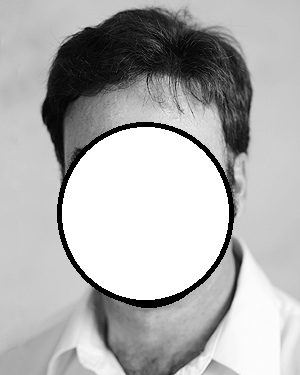
\includegraphics[width=1in,height=1.25in,clip,keepaspectratio]{author1.png}}]{First A. Author} received the B.S. and M.S. degrees in aerospace engineering from
the University of Virginia, Charlottesville, in 2001 and the Ph.D. degree in
mechanical engineering from Drexel University, Philadelphia, PA, in 2008.

From 2001 to 2004, he was a Research Assistant with the Princeton Plasma
Physics Laboratory. Since 2009, he has been an Assistant Professor with the
Mechanical Engineering Department, Texas A{\&}M University, College Station.
He is the author of three books, more than 150 articles, and more than 70
inventions. His research interests include high-pressure and high-density
nonthermal plasma discharge processes and applications, microscale plasma
discharges, discharges in liquids, spectroscopic diagnostics, plasma
propulsion, and innovation plasma applications. He is an Associate Editor of
the journal \emph{Earth, Moon, Planets}, and holds two patents.

Dr. Author was a recipient of the International Association of Geomagnetism
and Aeronomy Young Scientist Award for Excellence in 2008, and the IEEE
Electromagnetic Compatibility Society Best Symposium Paper Award in 2011.
\end{IEEEbiography}


\begin{IEEEbiography}[{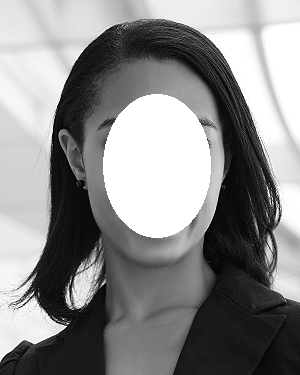
\includegraphics[width=1in,height=1.25in,clip,keepaspectratio]{author2.png}}]{Second B. Author} (M'76--SM'81--F'87) and all authors may include
biographies. Biographies are often not included in conference-related
papers. This author became a Member (M) of IEEE in 1976, a Senior
Member (SM) in 1981, and a Fellow (F) in 1987. The first paragraph may
contain a place and/or date of birth (list place, then date). Next,
the author's educational background is listed. The degrees should be
listed with type of degree in what field, which institution, city,
state, and country, and year the degree was earned. The author's major
field of study should be lower-cased.

The second paragraph uses the pronoun of the person (he or she) and not the
author's last name. It lists military and work experience, including summer
and fellowship jobs. Job titles are capitalized. The current job must have a
location; previous positions may be listed
without one. Information concerning previous publications may be included.
Try not to list more than three books or published articles. The format for
listing publishers of a book within the biography is: title of book
(publisher name, year) similar to a reference. Current and previous research
interests end the paragraph.

The third paragraph begins with the author's
title and last name (e.g., Dr.\ Smith, Prof.\ Jones, Mr.\ Kajor, Ms.\ Hunter).
List any memberships in professional societies other than the IEEE. Finally,
list any awards and work for IEEE committees and publications. If a
photograph is provided, it should be of good quality, and
professional-looking. Following are two examples of an author's biography.
\end{IEEEbiography}

\newpage

%If you do not have or do not want to include a photo, you can use IEEEbiographynophoto as shown below:

\begin{IEEEbiographynophoto}{Third C. Author, Jr.} (M'87) received the B.S. degree in mechanical
engineering from National Chung Cheng University, Chiayi, Taiwan, in 2004
and the M.S. degree in mechanical engineering from National Tsing Hua
University, Hsinchu, Taiwan, in 2006. He is currently pursuing the Ph.D.
degree in mechanical engineering at Texas A{\&}M University, College
Station, TX, USA.

From 2008 to 2009, he was a Research Assistant with the Institute of
Physics, Academia Sinica, Tapei, Taiwan. His research interest includes the
development of surface processing and biological/medical treatment
techniques using nonthermal atmospheric pressure plasmas, fundamental study
of plasma sources, and fabrication of micro- or nanostructured surfaces.

Mr. Author's awards and honors include the Frew Fellowship (Australian
Academy of Science), the I. I. Rabi Prize (APS), the European Frequency and
Time Forum Award, the Carl Zeiss Research Award, the William F. Meggers
Award and the Adolph Lomb Medal (OSA).
\end{IEEEbiographynophoto}

\EOD

\end{document}
